\scanpage{56}
% archive sheet number: 55
% letterhead
U N I V E R S I T E\\
DES SCIENCES ET TECHNIQUES\\
DU LANGUEDOC\\
\texttt{-{}-{}-{}-{}-{}-{}-{}-{}-{}-{}-{}-}\\
Service de la Scolarité\\
MR/GJ\\
Diffusion : Liste H\\
N° 3758

MONTPELLIER, le 15 Juin 1978

% printed form
\uline{AVIS DE SOUTENANCE D'UNE THESE DE DOCTORAT D'ETAT}

\uline{Nom et prénom du candidat} : WALTER Philippe

\uline{Titre de la thèse} : Recherches écologiques et biologiques sur les Scarabéides Coprophages d'une savane du Zaïre.

\uline{Date, heure et lieu de soutenance prévus} : 3 JUILLET 1978 à 9 Heures 30 mn\\
Salle de cours n° 6, U.S.T.L.

\uline{Nom du Directeur de thèse} : Monsieur le Professeur Renaud PAULIAN.

\uline{Désignation du laboratoire où la thèse est préparée} : Zoologie (Professeur LEGENDRE)

\uline{Résumé de la thèse} : Les recherches ont été effectuées sur le Plateau Bateke zaïrois. Les résultats sont présentés en trois parties :

1) le peuplement (composition d'ensemble, aspects biogéographiques, répartition dans les différentes formations végétales, fluctuations des densités de population, sex-ratio)

2) observations autoécologiques et biologiques (préférences trophiques, heures d'activité, éthologie)

3) morphologie larvaire : description détaillée de 12 larves.

\uline{Durée approximative des recherches ayant abouti à la thèse} : 5 ans 1/2.

\uline{Noms des Rapporteurs} :

\diagram{\begin{tabular}{@{}l p{.70\linewidth}@{}}
PAULIAN R. & , Professeur, Zoogéographie, Rectorat BORDEAUX\\
LAMOTTE M. & , Professeur, Ecologie, Ecole Normale Supérieure PARIS\\
LEGENDRE R. & , Professeur, Zoologie Ecologie, U.S.T.L.
\end{tabular}}

\uline{Composition du jury} :

\diagram{\begin{tabular}{@{}l p{.70\linewidth}@{}}
LEGENDRE R. & , Professeur, Zoologie Ecologie, U.S.T.L.\newline (Président)\\
PAULIAN R. & , Professeur, Zoogéographie, Rectorat BORDEAUX\\
LAMOTTE M. & , Professeur, Ecologie, Ecole Normale Supérieure PARIS\newline (Membres extérieurs choisis en raison de leur compétence scientifique)\\
EUZET L. & , Professeur, Parasitologie, U.S.T.L.\newline (Membre étranger à la spécialité du candidat)\\
LUMARET J.-P. & , Maître-assistant, Biogéographie, Univ. MONTPELLIER III.\\
BARAUD J. & ., Professeur, Biochimie, Univ. BORDEAUX
\end{tabular}}

Le Secrétaire Général,\\
\handwritten{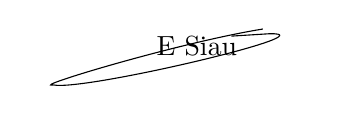
\begin{tikzpicture}[baseline=-.2ex,x=1cm,y=1cm]
\node at (1.86,.37) {\unsure{E Siau}};
\draw (.04,-.12) .. controls (-.28,-.16) and (1.64,.42) .. (2.70,.59);
\draw (.04,-.12) .. controls (.43,-.20) and (3.60,.55) .. (2.78,.53) -- (2.30,.50);
\end{tikzpicture}}\\
\uline{E. SIAU}

